\documentclass[a4paper,12pt]{article}

\usepackage[utf8]{inputenc}
\usepackage[T1]{polski}
\usepackage{helvet}
\usepackage{graphicx}
\usepackage{color}
\usepackage{xcolor}
\usepackage{geometry}
\usepackage{register}
\usepackage{listings}
\usepackage{caption}
\usepackage{makeidx}
\usepackage{longtable}
\usepackage{multirow}
\usepackage{wrapfig}


\geometry{hmargin={2cm, 2cm}, height=10.0in}
\DeclareCaptionFont{white}{\color{white}}
\DeclareCaptionFormat{listing}{\colorbox{gray}{\parbox{\textwidth}{#1#2#3}}}
\captionsetup[lstlisting]{format=listing,labelfont=white,textfont=white}
\lstset{ %
language=Verilog,               % choose the language of the code
basicstyle=\footnotesize,       % the size of the fonts that are used for the code
numbers=left,                   % where to put the line-numbers
numberstyle=\footnotesize,      % the size of the fonts that are used for the line-numbers
stepnumber=1,                   % the step between two line-numbers. If it's 1 each line
                                % will be numbered
numbersep=5pt,                  % how far the line-numbers are from the code
backgroundcolor=\color{white},  % choose the background color. You must add \usepackage{color}
showspaces=false,               % show spaces adding particular underscores
showstringspaces=false,         % underline spaces within strings
showtabs=false,                 % show tabs within strings adding particular underscores
frame=single,	                % adds a frame around the code
tabsize=2,	                % sets default tabsize to 2 spaces
%captionpos=b,                   % sets the caption-position to bottom
breaklines=true,                % sets automatic line breaking
breakatwhitespace=false,        % sets if automatic breaks should only happen at whitespace
title=\lstname,                 % show the filename of files included with \lstinputlisting;
                                % also try caption instead of title
escapeinside={\%*}{*)},         % if you want to add a comment within your code
morekeywords={*,...}            % if you want to add more keywords to the set
}

\lstloadlanguages{ Verilog }

\makeindex

\begin{document}

% =====  STRONA TYTULOWA PRACY MAGISTERSKIEJKIEJ ====
% ostatnia modyfikacja: 2009/07/01, K. Malarz

\thispagestyle{empty}
%% ------------------------ NAGLOWEK STRONY ---------------------------------
\begin{figure}
\vspace{-13cm}
\hspace{-4cm}

\includegraphics[height=29.3cm]{grafika/agh_nzw_a_pl_1w_wbr_cmyk.pdf}\\
\vspace{-13.9cm}
\end{figure}
\rule{26mm}{0pt}
{\large\textsf{Wydział Fizyki i Informatyki Stosowanej}}\\
\rule{\textwidth}{3pt}\\
\rule[2ex]
{\textwidth}{1pt}\\
\vspace{7ex}
\begin{center}
{\LARGE \bf \textsf{Praca magisterska}}\\
\vspace{13ex}
% --------------------------- IMIE I NAZWISKO -------------------------------
{\bf\Large\textsf{Krystian Wojtas}}\\
\vspace{3ex}
{\sf \small kierunek studiów:} {\bf\small\textsf{informatyka stosowana}}\\
\vspace{1.5ex}
{\sf \small kierunek dyplomowania:} {\bf\small\textsf{metody numeryczne}}\\
\vspace{10ex}
%% ------------------------ TYTUL PRACY --------------------------------------
{\bf \huge \textsf{Oprogramowanie sprzętu laboratoryjnego dedykowanego dla przedmiotu "Projektowanie Systemów Cyfrowych"}}\\
\vspace{6ex}
%% ------------------------ OPIEKUN PRACY ------------------------------------
{\Large Opiekun: \bf \textsf{dr inż. Krzysztof Świentek}}\\
\vspace{28ex}
{\large \bf \textsf{Kraków, czerwiec 2012}}
\end{center}
%% =====  STRONA TYTUŁOWA PRACY MAGISTERSKIEJKIEJ ====

\newpage

%% =====  TYŁ STRONY TYTUŁOWEJ PRACY MAGISTERSKIEJKIEJ ====
{\sf Oświadczam, świadomy(-a) odpowiedzialności karnej za poświadczenie nieprawdy, że niniejszą pracę dyplomową wykonałem(-am) osobiście i samodzielnie i  nie korzystałem(-am) ze źródeł innych niż wymienione w pracy.}

\vspace{14ex}

\begin{center}
\begin{tabular}{lr}
~~~~~~~~~~~~~~~~~~~~~~~~~~~~~~~~~~~~~~~~~~~~~~~~~~~~~~~~~~~~~~~~~ &
................................................................. \\
~ & {\sf (czytelny podpis)}\\
\end{tabular}
\end{center}

\newpage
\noindent
Na kolejnych dwóch stronach proszę dołączyć kolejno recenzje pracy popełnione przez Opiekuna oraz Recenzenta (wydrukowane z systemu MISIO i podpisane przez odpowiednio Opiekuna i Recenzenta pracy). Papierową wersję pracy (zawierającą podpisane recenzje) proszę złożyć w dziekanacie celem rejestracji co najmniej na tydzień przed planowaną obroną.

\newpage
\noindent
Na kolejnych dwóch stronach proszę dołączyć kolejno recenzje pracy popełnione przez Opiekuna oraz Recenzenta (wydrukowane z systemu MISIO i podpisane przez odpowiednio Opiekuna i Recenzenta pracy). Papierową wersję pracy (zawierającą podpisane recenzje) proszę złożyć w dziekanacie celem rejestracji co najmniej na tydzień przed planowaną obroną.


\vspace{85mm}
\newpage
\tableofcontents

\newpage
\section{Cel pracy}

\begin{figure}[htb]
   \centering
   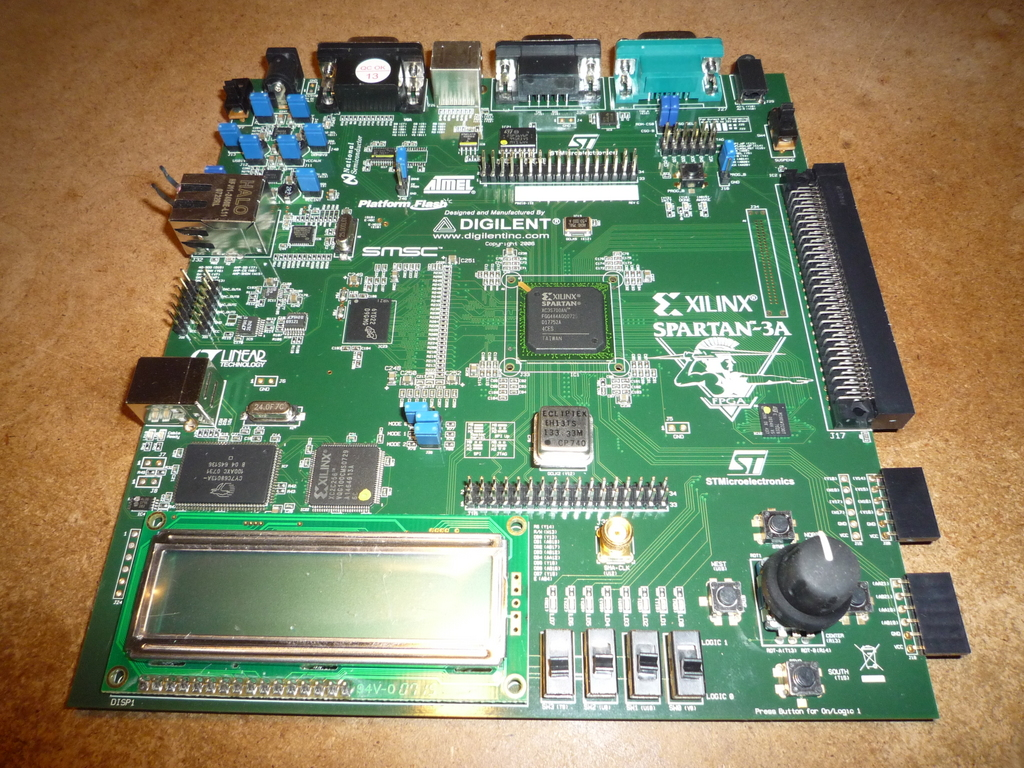
\includegraphics{grafika/spartan3an.jpg}
   \caption{Xilnix Spartan-3AN Starter Kit}
\end{figure}

Celem pracy jest oprogramowanie za pomocą języka opisu sprzętu (Verliog) układów używanych podczas zajęć laboratoryjnych z Projektowanie Systemów Cyfrowych. Praca polegałaby na przygotowaniu zestawu syntezowalnych bloków HDL do wszystkich elementów płytki „Xilnix Spartan-3AN Starter Kit” (www.xilinx.com/products/devkits/HW-SPAR3AN-SK-UNI-G.htm). Dodatkowo należy opracować modele behawioralne służące do testowania poprawności kodu (poszczególnych modułów sprzętu) tworzonego przez studentów podczas zajęć. Podsumowaniem całości ma być projekt kompleksowo demonstrujący możliwości wyżej wspomnianego sprzętu.

Utworzone moduły behawioralne muszą (wiernie) odzwierciedlać zachowania układów występujących na płytce.
Znajdą wtedy zastosowanie w uruchamianych symulacjach przebiegów czasowych danej konfiguracji układu programowalnego FPGA. Dzięki nim możliwe będzie stwierdzenie czy dla zsyntetyzowanej konfiguracji stany linii FPGA prowadzące do konkretnego układu płytki przebiegają poprawnie i czy zachodzi pożądana komunikacja poprzez generowanie przez te moduły stosownych komunikatów. W ten sposób studenci będą mogli testować poprawność działania utworzonej przez siebie konfiguracji bez fizycznego dosępu do sprzętu.
%zsyntetysowanej/wysyntetyzowanej


\newpage
\section{Projekty}
Każdy z symulowanych układów jest osobnym symulowalnym jak również syntezowalnym projektem środowiska Xilinx ISE. Projekty objęte są rozproszonym systemem kontroli wersji GIT, każdy jest jego osobnym podmodułem spajanym repozytorium superprojektu.

\subsection{Moduły ogólnego zastosowania}
Moduły ogólnego zastosowania, współdzielone pomiędzy projektami położone są w folderze nazwanym generic.

\subsubsection{Zegar}
Jest to moduł niezbędny do symulacji, wprowadza prostokątną linie zegarową.
\lstinputlisting[label=Zegar,caption=Clock.v]{zrodla/generic/sim/Clock.v}

\subsubsection{Reset}
Moduł na chwilę podnosi linię resetu.
\lstinputlisting[label=Reset,caption=Reset.v]{zrodla/generic/sim/Reset.v}

\subsubsection{Funkcja logarytmiczna}
Funkcja ta jest bardzo pomocna w ustaleniu szerokości deklarowanego rejestru na podstawie górnego zakresu liczb przez niego zapamietywanych. Wartość funkcji obliczana jest na etapie elaboracji.
\lstinputlisting[label=log2,caption=log2.v]{zrodla/generic/log2.v}

\subsubsection{Licznik}
Zastosowanie licznika powtarza się bardzo często. Dlatego wydzilony on został do osobnego ogólnego modułu.
\lstinputlisting[label=licznik,caption=Counter.v]{zrodla/generic/Counter.v}

\subsubsection{Rejestr przesuwny}
Rejestr przesuwny zapisuje daną wejsciową z interfejsu równoległego do swojego wewnętrznego rejestry w momencie, gdy zauważy podiesioną flagę 'set'. Jeśli flagi właczenia 'en' oraz działania 'tick' są ustawione, wtedy moduł rejest przesuwa, wstawiając dostarczony bit 'rx' w puste miejsce. Wyjściowy bit 'tx' zawsze wskazuje na bit z końca rejestru.
\lstinputlisting[label=rejestr,caption=Shiftreg.v]{zrodla/generic/Shiftreg.v}

\subsubsection{Serializacja}
Zadaniem modułu jest serializacja tj. przesłanie danych dostarczonych naraz interfejsem równoległym po kolei bit po bicie w takt zegara lub operacja desarializaj tj. operacja odwrotna. Moduł wykorzystuje zaprezentowany rejestr przesuwny oraz licznik.
\lstinputlisting[label=serial,caption=Serial.v]{zrodla/generic/Serial.v}

\subsubsection{SPI}
Serial Peripheral Interface jest popularnym sprzętowym interfejsem komunikacji. Jest on wyjaśniony w części poświęconej DAC-owi. Wykorzystuje moduł serializacji dodając jedynie funcjonalność lini Chip Select.
\lstinputlisting[label=spi,caption=Spi.v]{zrodla/generic/Spi.v}

\subsubsection{Generator impulsów}
Zadaniem generatorota impulsów jest wytwarzanie impulsów jak najbliższe pożadanemu okresowi.
\lstinputlisting[label=BaudRateGenerator,caption=BaudRateGenerator.v]{zrodla/generic/BaudRateGenerator.v}

\newpage
\section{DAC}
Zadaniem konwertera cyfrowo-analogowego jest przetwarzanie przekazanych mu kolejnych liczb binarnych na ich analogowe odpowiedniki realizowane jako wartość napięcia na jego pinie wyjściowym w zakresie napięcia maksymalnego $V_{ref}$.

Obsługiwany przez przetwornik zakres liczb binarnych jest dokładnością przetwornika. Występujący na płytce układ scalony LTC2624 ma zatopione 4 przetworniki DAC o dokładności 12-bitowej. Wszystkie przetworniki domyślnie mają wartość napięcia maksymalnego $V_{ref} = 3.3V$, jednak dla dwóch z nich wartość tą można indywidualnie ustawić komunikując się z układem wzmacniaczy zawartych w kostce LP3906. Wartości napięć wyjściowych podaje wzór
$$V_{out} = \frac{D[11:0]}{4096}  V_{ref}$$

\subsection{Komunikacja}

\subsubsection{SPI}
Układ LTC2624 zaimplementowaną ma logikę komunikacji w standardzie magistrali Serial Peripheral Interface.

\begin{figure}[htb]
   \centering
   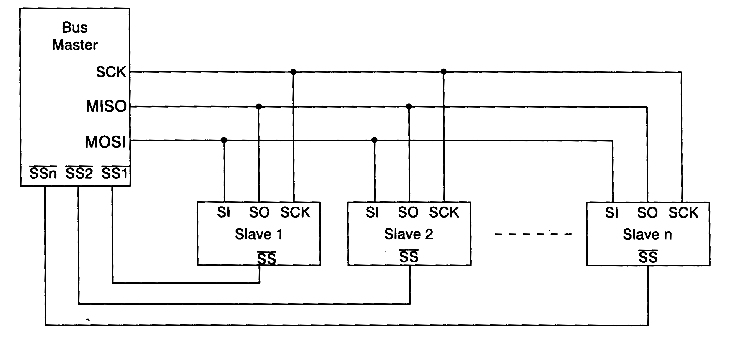
\includegraphics[width=15cm]{grafika/spi.jpg}
   \caption{SPI}
\end{figure}

Na magistrali występuje jeden układ nadrzędny - Master oraz co najmniej jeden Slave.
Master generuje zegar na linii SCK.
Master wysyła dane do Slavów szeregowo linią MOSI, Slavy odsyłają dane linią MISO. Transmisja jest fullduplexowana - przesył w obu kierunkach poszczególnych bitów następuje równocześnie w takt zegara.
Między układami współdzielone są linie zegara oraz danych. Odseparowane natomiast są linie CS poszczególnych slavów - wywołanie niskiego potencjału przez mastera aktywuje danego slava do uczestnictwa w wymianie danych.


\newpage
\subsubsection{Połączenia}

\begin{figure}[htb]
   \centering
   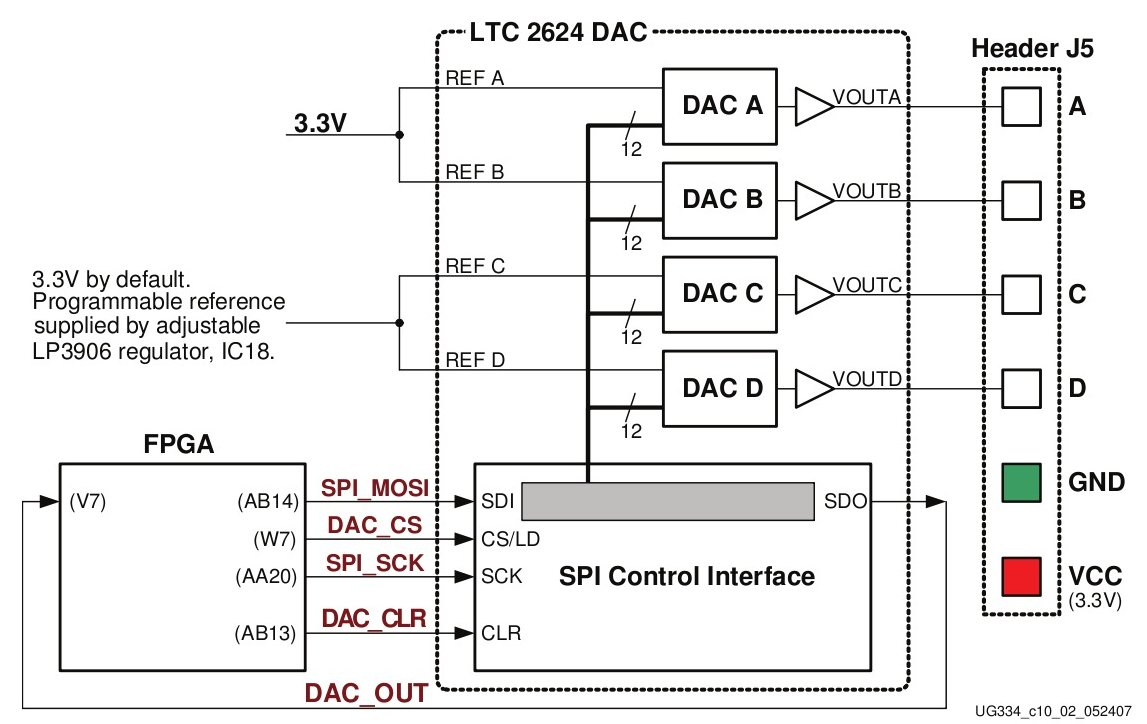
\includegraphics[width=15cm]{grafika/dac.jpg}
   \caption{Schemat polaczen ukladow LTC2624 i FPGA}
\end{figure}

Przed pierwszym użyciem należy układ zresetować chwilowo obniżając stan linii DAC\_CLR.

Na linie SPI\_SCK należy podać zegar o częstotliwości nie przekraczającej 50Mhz. Obniżając stan linii DAC\_CS rozpoczynamy komunikację z układem. Wtedy w takt zegara przesyłamy szeregowo do niego kolejne bity danych linią SPI\_MOSI. LTC2624 ładuje kolejne przesyłane bity do swojego rejestru przesuwnego na narastającym zboczu zegara oraz zwraca swoją poprzednią zawartość linią DAC\_OUT na opadającym zboczu. Natychmiast po wysłaniu kompletu danych należy koniecznie podnieść stan linii DAC\_CS zakańczając transmisję.

\begin{figure}[htb]
   \centering
   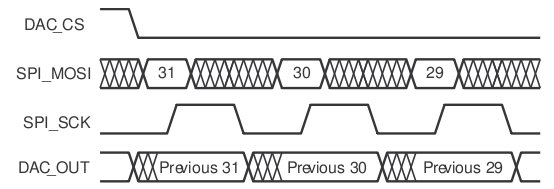
\includegraphics[width=15cm]{grafika/dac-waveform.jpg}
   \caption{Wykres stanow linii}
\end{figure}


\newpage
\subsubsection{Protokół komunikacji}

\begin{figure}[htb]
  \centering
	\begin{register}{H}{Przesylana ramka}{a}
	\label{dacprotocol}%
	\regfield{Nieistotne}{8}{24}{10000000}%
	\regfield{Komenda}{4}{20}{1100}%
	\regfield{Adres}{4}{16}{1111}%
	\regfield{Wartosc}{12}{4}{100000000000}%
	\regfield{Nieistotne}{4}{0}{0001}%
	\end{register}
\end{figure}

Dane przesyłane do układu LTC2624 są 32-bitową ramką uwidocznioną powyższym polem bitowym. Bity wysyła się kolejno zaczynając od najstarszego. Transmisja zaczyna się ośmioma nic nie znaczącymi bitami. Po nich wysyłane jest 4-bitowe pole komendy - typowo o wartości $0011$, co oznacza natychmiastowe wystawienie zadanej wartości napięcia. Następnie podawany jest adres konwertera według poniższej tabeli

\begin{figure}[htb]
  \centering
	\begin{tabular}{|c|c|c|c|l|}
	  \multicolumn{1}{r}{19}&\multicolumn{1}{r}{}&\multicolumn{1}{r}{}&\multicolumn{1}{r}{16}&\multicolumn{1}{l}{Adres}\\
		\hline
		0&0&0&0 & DAC A\\
		\hline
		0&0&0&1 & DAC B\\
		\hline
		0&0&1&0 & DAC C\\
		\hline
		0&0&1&1 & DAC D\\
		\hline
		1&1&1&1 & Wszystkie\\
		\hline
	\end{tabular}
\end{figure}

Trzecie pole jest 12-bitową wartością binarną odpowiadającą wystawianemu napięciu. Ramka kończy się 4 nieistotnymi bitami. W przykładzie na wszystkich konwerterach pojawiłaby się połowa z ustawionych zakresów napięć.



\subsection{HDL}
\lstinputlisting[caption=Top.v]{../projects/dac/Top.v}
\lstinputlisting[label=Controller,caption=Controller.v]{../projects/dac/Controller.v}
\lstinputlisting[label=DacSpi,caption=DacSpi.v]{../projects/dac/DacSpi.v}

%\newpage
\subsection{Moduł behawioralny}
Wykonana została wzorcowa konfiguracja FPGA poprawnie ustawiająca DAC-i. Przedstawiona symulacja pokazuje wykres przebiegów czasowych linii prowadzących do układu DAC. Układ taktowany jest zegarem 50Mhz pochodzącym z kwarcu dostępnego na płytce. Przesyłana ramka jest przykładem z poprzedniego rozdziału - połowa zakresów napięć wystawiana na wszystkich dac-ach. Pola z bitami nieistonymi są tak ustawione aby pojedynczymi, skrajnymi pikami pokazywały początek i koniec ramki.

\begin{figure}[htb]
   \centering
   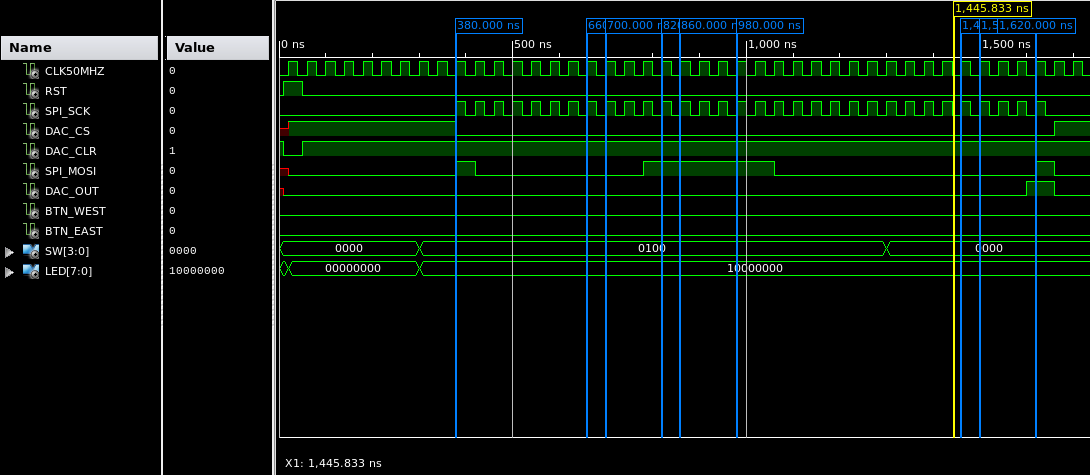
\includegraphics[width=13cm]{grafika/toptest-fastdac-110.png}
\end{figure}


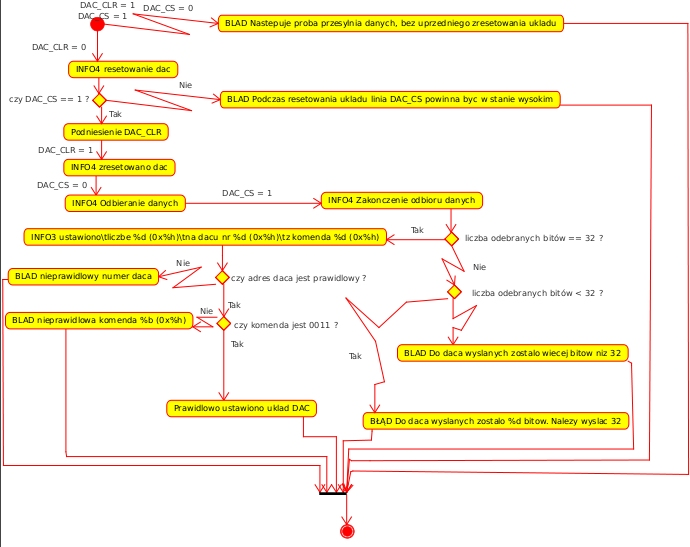
\includegraphics[width=15cm]{grafika/dac-uml.jpg}

\lstinputlisting[label=dac,caption=dacLTC2624behav.v]{zrodla/dacLTC2624-behav.v}


\newpage
\section{Rotor}

Płytka Spartan 3AN jest wyposażona w obrotowy przełącznik o dwóch wyprowadzeniach do FPGA. W stanie jałowym są one przyłączone do wysokiego potencjału. Mechaniczne obracanie pokrętła powoduje zwieranie styków na liniach i uziemienie napięcia. Kierunek obrotu wyznacza linia, która wcześniej się zewrze do masy lub, co jest ekwiwalentne, wcześniej wróci do stanu jałowego.

\begin{figure}[htb]
   \centering
   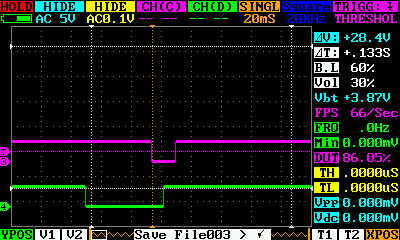
\includegraphics[width=13cm]{grafika/dso/rotor-w-prawo-jeden.png}
   \caption{Obrót w kierunku zgodnym z ruchem wskazówek zegara. Fioletowa linia wykreśla sygnał $rota$.}
\end{figure}

\begin{figure}[htb]
   \centering
   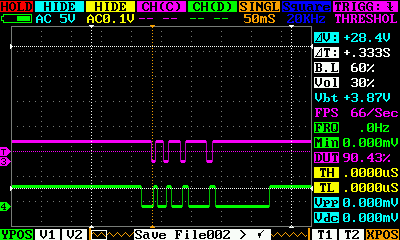
\includegraphics[width=13cm]{grafika/dso/rotor-w-prawo-wiele.png}
   \caption{Kilka obrotów następujących po sobie}
\end{figure}

\subsection{Aplikacja}

FPGA po skonfigurowaniu lub zresetowaniu zapala jedną diode, piątą lub szóstą w szeregu. Obrót rotora powoduje przesunięcie stanu wszystkich diód o jedną pozycję w lewo lub w prawo w zależności od kierunku obrotu. Pozycje skrajne się cyklicznie uzupełniają. Rotor można także nacisnąć, co spowoduje zmiane stanu pierwszej diody na przeciwny.

\subsection{Synteza}

\subsubsection{Warstwa wierzchnia}

FPGA korzysta z wyprowadzeń zegara, dolnego przycisku resetu, $ROT\_CENTER$ jest do obsługi wciśnięć. $ROT\_A$ oraz $ROT\_B$ są połączeniami do pokrętła. Są też wyprowadzenia dla diód i dodatkowe połączenia pokrętła na oscyloskop.
\begin{lstlisting}[label=Rs232Tx,caption=Rs232Tx.v,firstnumber=14]
module Top (
    input        CLK50MHZ,
    input        RST,
    // rotor control
    input        ROT_CENTER,
    input        ROT_A,
    input        ROT_B,
    // leds
    output [7:0] LED,
    // debug
    output       DEBUG_A,
    output       DEBUG_B
    );
\end{lstlisting}
Przycisk $ROT\_CENTER$ jest pozbawiany drgań styków dzięki przeprowadzeniu przez $Debouncer$-a. Zainstancjonowane są tu także moduły $Rotor$-a oraz $Controller$-a. Wyprowadzenia debugera to przypisania ciągłe na odpowiadające połączenia obrotu.

\subsubsection{Rotor}
$Rotor$ otrzymuje bezpośrednio sygnały o mechanicznych obrotach pokrętła i je interpretuje, w wyniku czego sygnalizuje wykryte obroty wraz z ich rozpoznanym kierunkiem.
\begin{lstlisting}[label=Rotor,caption=Rotor.v]
module Rotor(
    input clk,
    input rst,
    // inputs
    input rota,
    input rotb,
    // one pulse output direction signals
    output left,
    output right
);
\end{lstlisting}

Dla zobrazowanie dalszych zależności między sygnałami, zamieszczony jest zrzut z symulacji.
\begin{figure}[htb]
   \centering
   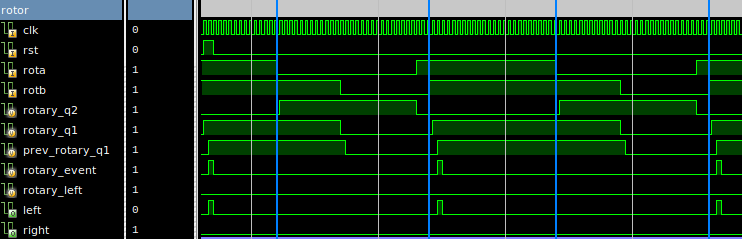
\includegraphics[width=15cm]{grafika/rotor.png}
   \caption{Symulacja sygnałów rotora}
\end{figure}

Rejestry pomocnicze zatrzaskują stan linii $rotb$. $rotary\_q1$ gdy wyprowadzenia pokrętła są zgodne, natomiast $rotary\_q2$ gdy są przeciwne.
\begin{lstlisting}[label=Rotor,caption=Rotor.v,firstnumber=12]
    reg rotary_q1 = 1'b0;
    always @(posedge clk)
        if(rota ~^ rotb)
            rotary_q1 <= rotb;

    reg rotary_q2 = 1'b0;
    always @(posedge clk)
        if(rota ^ rotb)
             rotary_q2 <= rotb;
\end{lstlisting}

Dodatkowy rejestr $prev\_rotary\_q1$ przechowuje wartość $rotary\_q1$ z poprzedniej chwili. To umożliwia wykrycie zbocza narastającego $rotary\_q1$, czyli momentu gdy obrót się skończył i oba wyprowadzenia pokrętła są ponownie wysokie w stanie jałowym.

Pogląd na kierunek obrotu daje drugi rejestr pomocniczy $rotary\_q2$. Linie pokrętłą nie kończą wysterowywania obrotu jednocześnie. Kolejność powrotów mówi o kierunku obrotu. $rotary\_q2$ zachowa stan $rotb$ w chwili pierwszego powrotu. Wystarczy teraz sprawdzić zachowany stan $rotary\_q2$, by odpowiedzieć czy ona wróciła pierwsza, co implikowałoby obrót w prawo - zgodny z ruchem wskazówek zegara.
\begin{lstlisting}[label=Rotor,caption=Rotor.v,firstnumber=22]
    reg prev_rotary_q1 = 1'b0;
    reg rotary_event = 1'b0;
    reg rotary_left = 1'b0;
    always @(posedge clk) begin
        prev_rotary_q1 <= rotary_q1;
        if(~prev_rotary_q1 && rotary_q1) begin
            rotary_event <= 1'b1;
            rotary_left <= rotary_q2;
        end else
            rotary_event <= 1'b0;
    end

    assign left = rotary_event & ~rotary_left;
    assign right = rotary_event & rotary_left;

endmodule
\end{lstlisting}

\subsubsection{Kontroler}

Kontroler operuje na rejestrze, który powiązany jest z diodami led na płytce. Po świeżej konfiguracji płytki świeci się dioda piąta. Przycisk resetu ustawia jedynie szóstą. Przycisk centralny pokrętła zmieni stan diody pierwszej na przeciwny. Kontroler dostaje też impulsy $left$ oraz $right$ informujący o zajściu obrotu i jego kierunku. Wtedy przesuwa bity rejestru w wyznaczonym kursie.
\begin{lstlisting}[label=Controller,caption=Controller.v]
module Controller(
         input clk,
         input rst,
         // tick inputs
         input center,
         input left,
         input right,
         //  leds
         output reg [7:0] leds = 8'b0001_0000
    );

    always @(posedge clk)
        if(rst)           leds <= 8'b0010_0000;
        else if(center)   leds[0] <= ~leds[0];
        else if(left)     leds <= { leds[6:0], leds[7] };
        else if(right)    leds <= { leds[0], leds[7:1] };

endmodule
\end{lstlisting}

\subsection{Symulacja}
Moduły testowe jedynie symulują obracanie pokrętła przez użytkownika poprzez wysterowanie jego sygnałów. Moduł najwyższy symulacji jedynie zapewnia zainstancjonowanie zegara, resetu, modułu syntezowalnego i testowego odpowiednika pokrętła.

\subsubsection{Przypadek testowy}


\begin{lstlisting}[label=TopTestBench,caption=TopTestBench.v]
module TopTestBench #(
   LOGLEVEL = 3,
   LOGLEVEL_BEHAV = 3,
   LOGLEVEL_BEHAV_CENTER = 3,
   LOGLEVEL_BEHAV_ROTA = 3,
   LOGLEVEL_BEHAV_ROTB = 3
) (
   // rotor control
   output ROT_CENTER,
   output ROT_A,
   output ROT_B
);
\end{lstlisting}
On z kolei instancjuje $Rotor\_behav$ i operuje pokrętłem poprzez jego zestaw zadań.
\begin{lstlisting}[label=TopTestBench,caption=TopTestBench.v,firstnumber=37]
      // kilka ruchow
      rotor_behav.turn_left();
      rotor_behav.turn_left();
      rotor_behav.press_center();
      rotor_behav.turn_right();
\end{lstlisting}

\begin{lstlisting}[label=Rotor_behav,caption=Rotor\_behav.v]
   task turn_left();
      begin
         ..
         // rozpoczecie skretu w lewo
         set_rota.low_during( 250 );
         set_rotb.low_during( 300 );

         // konczenie skretu w lewo
         set_rota.high_during( 50 );
         set_rotb.high_during( 500 );
         ..
      end
   endtask
\end{lstlisting}


\begin{lstlisting}[label=Rotor_behav,caption=Rotor\_behav.v]
   task turn_right();
      begin
         ..
         // rozpoczecie skretu w prawo
         set_rotb.low_during( 250 );
         set_rota.low_during( 300 );

         // konczenie skretu w prawo
         set_rotb.high_during( 50 );
         set_rota.high_during( 500 );
         ..
      end
   endtask
\end{lstlisting}



\begin{lstlisting}[label=Rotor_behav,caption=Rotor\_behav.v]
   task press_center();
      begin
         ..
         set_center.high_during( 400 );
         set_center.low_during( 200 );
         ..
      end
   endtask
\end{lstlisting}


\newpage
\section{Rs232}

Rs232 jest asynchronicznym, szeregowym standardem komunikacyjnym. Zdefiniowane są osobne linie do wysyłanych i odbieranych danych. Szybkość transmisji ustala się ręcznie w urządzeniach końcowych.

Stanem wysokim określony jest stan bezczynności. Nadawanie danych rozpoczyna się od opuszczenia linii $tx$ na okres jednego bitu tzw. startowego. Natępnie przesyłane są kolejne bity danych i kończone są wysokim bitem stopu. Standard przewiduje możliwy bit parzystości poprzedzający stop.

\subsection{Aplikacja}
Zaimplementowana aplikacja oczekuje wysłania bajtu danych przez urządzenie po drugiej stronie kabla, po czym mu go odsyła w niezmienionej postaci. Działa jak zwykłe echo. Pracuje z prędkością 115200 bitów na sekundę. Nie implementuje bitu parzystości.

\subsection{Synteza}

\subsubsection{Warstwa wierzchnia}
\iffalse
\subsubsection{Powierzchnia}
\fi
Moduł najwyższy w zasadzie przepuszcza wszystkie połączenia do właściwego modułu echa. Jedynie wyprowadza dodatkowo stan linii komunikacyjnych na złącze oscyloskopu do łatwej analizy. Natomiast moduł echa instancjuje część odbierającą i transmitującą dane oraz je łączy.
\lstinputlisting[caption=Rs232Echo.v]{../projects/rs232/Rs232Echo.v}


\subsubsection{Transmisja}
Transmiter jest prostszy, zatem od niego warto zacząć. Należy przekazać mu w parametrach taktowanie zegara podstawowego płytki oraz zakładaną prędkość pracy. Aby z modułu skorzystać wystarczy podsunąć wysyłany bajt połączeniem $TxD\_data$, po czym podnieść na jeden cykl $TxD\_start$. Wtedy zacznie formować stan linii wyjściowej $TxD$ poprzez serializacje dostarczonego bajtu wraz z dodatkowymi skrajnymi bitami startu i stopu. Swoją zajętość sygnalizuje flagą $TxD\_busy$.
\begin{lstlisting}[label=Rs232Tx,caption=Rs232Tx.v]
module Rs232Tx
#(
   parameter FREQ = 50000000,   // 50MHz
   parameter BAUD = 115200      // 115 200 bounds/sec
) (
   input       CLK50MHZ,
   input       RST,
   input       TxD_start,
   input [7:0] TxD_data,
   output      TxD,
   output      TxD_busy
);
\end{lstlisting}

Zalecany standard 232 przewiduje tolerancję niedokładności zegara nie przekraczającą $5\%$ w dowolnym kierunku. Przy przesyłanych łącznie 10 bitach w pakiecie oznacza to rozjechanie się zegarów odbiornika i nadajnika maksymalnie o pół bitu. Prosty licznik oparty na zegarze podstawowym $50Mhz$ nie spełnia wymagań. Należy zachowywać resztę z dodawań po każdym przepełnieniu. Dlatego do wyznaczenia momentu nadania kolejnego bitu służy dedykowany moduł $BaudRateGenerator$ z wykalkulowaną inkrementacją.
\begin{lstlisting}[label=Rs232Tx,caption=Rs232Tx.v,firstnumber=14]
   `include "../../generic/log2.v"
   localparam N = log2(BAUD);

   wire        BaudTick;
   wire        TxD_ready;
   BaudRateGenerator #(
        .INC( ((BAUD<<(N-4))+(FREQ>>5))/(FREQ>>4) ), // = 302
        .N(N)
     ) baud115200 (
        .CLK50MHZ(CLK50MHZ),
        .RST(RST),
        .en(TxD_busy),
        .tick(BaudTick)
    );
\end{lstlisting}

Znany moduł do serializacji zajmuje sie wysyłaniem danych w takt sygnału generowanego przez $BaudRateGenerator$. Dane te należy otoczyć bitem startu i stopu oraz w całości zanegować dla spójności z jałową jedynką.
\begin{lstlisting}[label=Rs232Tx,caption=Rs232Tx.v,firstnumber=29]
    // START BIT, data, STOP BIT
    wire [9:0]  rs_data = { 1'b1, ~TxD_data, 1'b0 };
   // output TxD line should be high at idle
    wire        TxD_neg;
    Serial #(
        .WIDTH(10)
    ) Serial_ (
        .CLKB(CLK50MHZ),
        .RST(RST),
        // serial module interface
        .rx(1'b0),
        .tx(TxD_neg),
        .data_in(rs_data),
        .trig(TxD_start),
        .ready(TxD_ready),
        .tick(BaudTick)
    );

   assign TxD      = ~ TxD_neg;
   assign TxD_busy = ~ TxD_ready;

endmodule
\end{lstlisting}


\subsubsection{Odbiór}
Moduł odbiorczy podobnie ma parametryzowane zegar podstawowy płytki oraz szybkość pracy. Gdy odbierze nowe dane, wystawia je na wyjścia $RxD\_data$ oraz informuje o zdarzeniu flagą $RxD\_data\_ready$ przez jeden cykl.
\begin{lstlisting}[label=Rs232Rx,caption=Rs232Rx.v]
module Rs232Rx
#(
        parameter FREQ = 50000000,      // 50MHz
        parameter BAUD = 115200         // 115 200 bounds/sec
) (
        input        CLK50MHZ,
        input        RST,
        input        RxD,
        output [7:0] RxD_data,
        output       RxD_data_ready
);
\end{lstlisting}

Protokół jest asynchroniczny, więc sygnał zegarowy nie jest przekazywany, co utrudnia nieco odbiór. Linia $RxD$ jest próbkowana z trzykrotnie większą częstotliwością, a przyjęty odebrany bit jest wynikiem głosowania próbek. Podejście wymusza powołanie również szybszego modułu $BaudRateGenerator$-a.
\begin{lstlisting}[label=Rs232Rx,caption=Rs232Rx.v,firstnumber=13]
   `include "../../generic/log2.v"
   localparam N = log2(BAUD);

   wire              receving;
   wire              BaudTick3;
   BaudRateGenerator #(
        // 3 times oversampling
        .INC( ((BAUD*3<<(N-7))+(FREQ>>8))/(FREQ>>7) ), // = 2416
        .N(N)
    ) baud_115200x3 (
        .CLK50MHZ(CLK50MHZ),
        .RST(RST),
        .en(receving),
        .tick(BaudTick3)
    );

    wire        BaudTick;
    BaudRateGenerator #(
        .INC( ((BAUD<<(N-4))+(FREQ>>5))/(FREQ>>4) ), // = 302
        .N(N)
    ) baud_115200 (
        .CLK50MHZ(CLK50MHZ),
        .RST(RST),
        .en(receving),
        .tick(BaudTick)
    );
\end{lstlisting}

Tutaj instancjalizowany jest rejestr przesuwny dla próbek oraz kreowany układ głosujacy przypisaniem ciągłym.
\begin{lstlisting}[label=Rs232Rx,caption=Rs232Rx.v,firstnumber=40]
   wire [2:0]   rx3;
   Shiftreg #(
      .WIDTH(3)
   ) rx3_shitftreg (
           .CLKB(CLK50MHZ),
           .en(1'b1),
           .set(1'b0),
           .tick(BaudTick3),
           .rx(RxD),
           .data_in(3'b000),
           .data_out(rx3)
           );

   // Vote for rx value
   wire                    rx =
                           rx3 != 3'b000 &&
                           rx3 != 3'b001 &&
                           rx3 != 3'b010 &&
                           rx3 != 3'b100;
\end{lstlisting}

Serializer zajmuje się deserializacją napływających bitów pakietu. Bity początkowy startu i końcowy stopu zostają obcięte.
\begin{lstlisting}[label=Rs232Rx,caption=Rs232Rx.v,firstnumber=59]
   wire                    trig;
   wire                    ready;
   wire [9:0]              data_out;
   Serial #(
        .WIDTH(10)
    ) Serial_ (
        .CLKB(CLK50MHZ),
        .RST(RST),
        // serial module interface
        .rx(rx),
        .data_in(10'b0),
        .data_out(data_out),
        .trig(trig),
        .ready(ready),
        .tick(BaudTick)
    );

   // get rid of START and STOP bits
   assign RxD_data = data_out[8:1];
\end{lstlisting}

Konieczna jest maszyna stanów. Najpierw wyczekuje niskiego bitu startu, po czym odbiera pakiet i zgłasza jego przyjęcie. Cykl się powtarza.
\begin{lstlisting}[label=Rs232Rx,caption=Rs232Rx.v,firstnumber=79]
   localparam [1:0]
     WAIT_STARTBIT = 3'd0,
     START_RECEVING = 3'd1,
     RECEVING = 3'd2,
     RECEIVED = 3'd3;

   reg [2:0]               state = WAIT_STARTBIT;
   always @(posedge CLK50MHZ)
     if(RST)
       state <= WAIT_STARTBIT;
     else
       case(state)
         WAIT_STARTBIT:
           if(~RxD)
             state <= START_RECEVING;
         START_RECEVING:
             state <= RECEVING;
         RECEVING:
           if(ready)
             state <= RECEIVED;
         RECEIVED:
             state <= WAIT_STARTBIT;
       endcase

   assign       trig = (state == START_RECEVING);
   assign       RxD_data_ready = (state == RECEIVED);
   assign       receving = (state == RECEVING);

endmodule
\end{lstlisting}

\subsection{Symulacja}

Moduł symulacyjny wysyła serię bajtów wzorcowych, po czym oczekuje odesłania ich z powrotem.

Moduł najwyższy $TopTest$ kreuje instancje zegara, resetu, $Rs232$ i wierzchni moduł syntezowalny oraz zapewnia między nimi połączenia.


\subsubsection{Rs232}


$Rs232$ zawiera pamięć z napisem, który zamierza nadać, po czym odebrać.
\begin{lstlisting}[label=sim/Rs232,caption=sim/Rs232.v,firstnumber=28]
   localparam CHARS = 8;
   reg [7:0] mem [CHARS:0];
   initial begin
      mem[0] = "A";
      mem[1] = "G";
      mem[2] = "H";
      mem[3] = " ";
      mem[4] = "W";
      mem[5] = "F";
      mem[6] = "i";
      mem[7] = "I";
      mem[8] = "S";
   end
\end{lstlisting}

Nadawane są kolejno litery korzystając z zadania modułu zachowawczego.
\begin{lstlisting}[label=sim/Rs232,caption=sim/Rs232.v,firstnumber=42]
   integer j = 0;
   initial begin
      ..
      // wyslanie kolejnych liter napisu powitalnego
      for(j=0; j<CHARS; j=j+1) begin
         rs232_behav.transmit( mem[j] );
         ..
      end
   end
\end{lstlisting}

Śledzona jest linia $rx$, która to powinny wysłane dane otrzymać z powrotem w tej samej formie i porządku, co zostaje poddane weryfikacji.
\begin{lstlisting}[label=sim/Rs232,caption=sim/Rs232.v,firstnumber=64]
   integer k = 0;
   reg [7:0] byte_received = 8'd0;
   always @(negedge rx) begin
      if(inited) begin

         // odbior bajtu
         rs232_behav.receive( byte_received );
         ..

         // weryfikacja
         if( byte_received != mem[k] )
            if(LOGLEVEL >= 1)
               $display("%t\t ERROR [ %m ] \t Odebrany bajt %b 0x%h %d %s rozni sie od wyslanego wzorca %b 0x%h %d %s", $time, byte_received, byte_received, byte_received, byte_received, mem[k], mem[k], mem[k], mem[k]);

         // inkrementuj numer biezacego bajtu
         k = k + 1;
     end
  end
\end{lstlisting}


\subsubsection{Rs232 zachowawczo}

Moduł udostępnia zadania do wysyłania oraz odbierania danych. Zajmuje się formowanie ich w pakiety z doklejonymi bitami startu i stopu lub wyłuskiwaniem jego zawartości. Informuje o przebiegu swojej pracy z wybraną sześciostopniową dokładnością poziomu logowania.
\begin{lstlisting}[label=sim/Rs232 behav,caption=sim/Rs232 behav.v]
module Rs232_behav
#(
   // LOGLEVEL = 0
   //      bez zadnych komunikatow
   // LOGLEVEL = 1
   //      pokazuje bledy
   // LOGLEVEL = 2
   //      pokazuje ostrzezenia
   //
   // LOGLEVEL = 3
   //      informuje o wyslaniu/otrzymaniu pelnego bajtu
   // LOGLEVEL = 4
   //      informuje o wysylaniu/otrzymywaniu poszczegolnych bitow
   // LOGLEVEL = 5
   //      informuje o wyslaniu/otrzymywaniue start i stop bitow
   // LOGLEVEL = 6
   //      informuje o przeczekiwaniu tolerowanego przesuniecia zegara
   parameter LOGLEVEL=3,
   parameter LOGLEVEL_RX=3,
   parameter LOGLEVEL_TX=3,

   parameter BAUDRATE = 115_200
) (
   input rx,
   output tx
);
\end{lstlisting}

Wyliczone są czasy trwania pojedynczego bitu na podstawie żądanej prędkości transmisji oraz tolerancji na błąd przesunięcia zegara.
\begin{lstlisting}[label=sim/Rs232 behav,caption=sim/Rs232 behav.v,firstnumber=64]
   // czas jednego okresu przy zakladanej szybkosci
   localparam PERIOD = 1_000_000_000 / BAUDRATE;
   // tolerancja zegara
   localparam BITTOL = 0.05 * PERIOD;
\end{lstlisting}

Zadanie wysyłające przyjmuje bajt danych. Wysyła go w pętli poprzedzając bitem startu i zakańczając stopem.
\begin{lstlisting}[label=sim/Rs232 behav,caption=sim/Rs232 behav.v,firstnumber=64]
   // Zadanie wysyla przekazany bajt wraz z poprzedajacym bitem startu i nastepujacym stopu
   task transmit
   (
      input [7:0] byte_tosend
   );
      integer     i;
      begin
         ..
         set_tx.low_during( PERIOD );

         // Przekazany bajt
         for(i=0; i < 8; i=i+1) begin
            set_tx.state_during( PERIOD, byte_tosend[i] );
            ..
         end

         // Stop bit
         ..
         set_tx.high_during( PERIOD );
         ..
      end
   endtask
\end{lstlisting}

Zadanie odbierające dane symetrycznie do nadającego spodziewa się bitu startu, bajtu danych i stop bitu.
\begin{lstlisting}[label=sim/Rs232 behav,caption=sim/Rs232 behav.v,firstnumber=118]
   task receive
   (
      output reg [7:0] byte_received
   );
      integer i;
      reg startbit;
      reg stopbit;
      begin
         // Zaczekaj na start bit
         ..
         monitor_rx.wait_for_low();
         ..
         // Odbierz bit startu
         receive_bit( startbit );
         if(startbit != 1'b0)
            if(LOGLEVEL >= 1)
               $display("%t\t ERROR [ %m ] \t Bit startu powinien byc niski", $time);
         ..
         // Odbierz bajt danych
         for(i=0; i < 8; i=i+1) begin
            receive_bit( byte_received[i] );
            ..
         end

         // Odbierz oczekiwany stop bit
         ..
         receive_bit( stopbit );
         if(stopbit != 1'b1)
            if(LOGLEVEL >= 1)
               $display("%t\t ERROR [ %m ] \t Oczekiwany bit stopu powinien byc wysoki", $time);
         ..
      end
   endtask
\end{lstlisting}

Odbiór bitu realizowany jest w kolejnym dedykowanym zadaniu. Sprawdzane jest, czy linia $rx$ jest stabilna przez dlugość trwania okresu z wyłączeniem początkowego i końcowego możliwego błędu synchronizacji zegarów.
\begin{lstlisting}[label=sim/Rs232 behav,caption=sim/Rs232 behav.v,firstnumber=89]
   // Zadanie odbiera bit probkujac go 3 krotnie
   task receive_bit
   (
      output reg received
   );
      begin
         ..
         #(BITTOL);
         ..
         monitor_rx.ensure_same_during( (PERIOD-2*BITTOL) );
         ..
         received = rx;
         ..
         #(BITTOL);
         ..
      end
   endtask
\end{lstlisting}


\subsubsection{Wyjście}

\begin{verbatim}
96800000 INFO3 [ TopTest.rs232 ]  Wyslano bajt '01001000' (0x 48) (dec  72) (ascii H)
183600000 INFO3 [ TopTest.rs232 ]  Wyslano bajt '01000101' (0x 45) (dec  69) (ascii E)
183710000 INFO3 [ TopTest.rs232 ]  Odebrano bajt '01001000' (0x 48) (dec  72) (ascii H)
270400000 INFO3 [ TopTest.rs232 ]  Wyslano bajt '01001100' (0x 4c) (dec  76) (ascii L)
270570000 INFO3 [ TopTest.rs232 ]  Odebrano bajt '01000101' (0x 45) (dec  69) (ascii E)
\end{verbatim}

%% \subsubsection{HDL}
%% \lstinputlisting[caption=Top.v]{../projects/rs232/Top.v}
%% \lstinputlisting[label=Rs232Tx,caption=Rs232Tx.v]{../projects/rs232/Rs232Tx.v}
%% \lstinputlisting[label=Rs232Rx,caption=Rs232Rx.v]{../projects/rs232/Rs232Rx.v}

%% 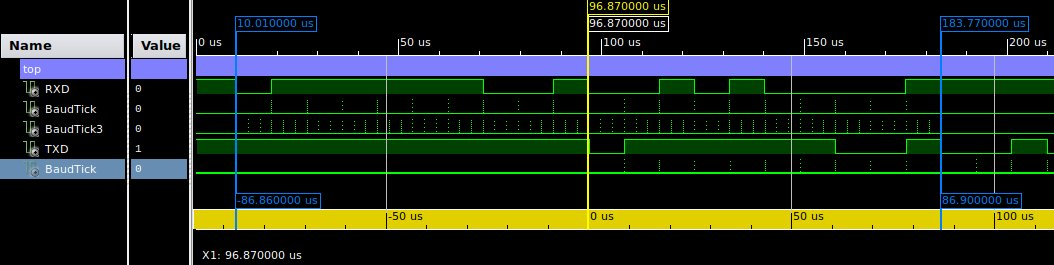
\includegraphics[width=15cm]{grafika/rs232-waveform.jpg}

%% \subsubsection{HDL}
%% \lstinputlisting[caption=Top.v]{../projects/rs232/sim/Rs232_behav.v}

\newpage
\section{VGA}
Standard VGA odpowiada za przesłanie obrazu do wyświetlacza przy ustalonych rozmiarach oraz częstotliwości odświeżania. Obraz przesyłany jest punkt po punkcie zwanych pikselami w porządku od lewej do prawej kolumny, zaczynając od górnego do dolnego wiersza.

Po przesłaniu każdego wiersza, następuje chwilowe obniżenie linii synchronizacyjnej $HSYNC$. Natomiast po przesłaniu całej ramki, chwilowo opuszczana jest linia $VSYNC$. W punktach tych i ich pewnym otoczeniu należy uzniemić linie kolorów.

Kolor pikseli określa złożenie nasycenia trzech podstawowych barw: czerwonej, zielonej i niebieskiej. Ich stan podawany jest osobnymi liniami analogowo wartościami napięcia z zakresu $0.0V - 0.7V$.

Płytka Spartan wykorzystuje po 4 cyfrowe wyjścia FPGA dla każdej z barw łączone w drabinki rezystorowe tworząc proste ADC.

\subsection{Aplikacja}
Zaprojektowana aplikacja pokazuje na ekranie przyłączonego wyświetlacza jeden z ośmiu kolorów. Użytkownik wybiera ulubiony kolor posługując się dwoma przyciskami. Jeden z nich przełącza kolor tła na następną dostępną barwe, drugi wraca do poprzedeniej. Końce listy dostępnych barw są połączone, próba wykroczenia poza nią powoduje płynne przejście na jej przeciwny koniec.

\subsection{Synteza}

\subsubsection{Połączenia}
\iffalse
\subsubsection{Top}
\fi
Moduł najwyższy przyjmuje sygnały zegarowy, resetu oraz dwóch przycisków służacych zmianie koloru wyświetlanego tła. Moduł wyprowadza sygnały synchronizacji ramek i kolumn oraz pożądany kolor podany poprzez trzy czterobitowe rejestry nasycenia czerwieni, błękitu i zieleni.

\begin{lstlisting}[label=Topvga,caption=Top.v]
module Top (
    input        CLK50MHZ,
    input        RST,
    // vga interface
    output [3:0] VGA_R,
    output [3:0] VGA_G,
    output [3:0] VGA_B,
    output       VGA_HSYNC,
    output       VGA_VSYNC,
    // color control
    input        BTN_NEXT,
    input        BTN_PREV,
);
\end{lstlisting}

Sygnały przycisków przewijania należy pozbawić drgań styków wykorzystując poznany moduł $Debouncer$. Następnie zostają zainstancjonowane moduły $Sync$ służący sychronizacji oraz $Controller$, który obsługuje przyciski i podaje wybrany kolor.

\subsubsection{Synchronizacja}
Zadaniem modułu synchronizacyjnego jest właściwe wytaktowanie linii zawiadamiających o początku nowej ramki lub nowej kolumny. Są to sygnały cyfrowe utrzymywane w stanie wysokim, w chwilach synchronizacji zostają obniżane. Domyślne parametry dostosowane są do przesyłania obrazu rozmiaru 640x480 pikseli przy częstotliwości odświeżania 60 Hz. Odmierzanie czasu przesyłu kolum  bazuje na podstawowym zegarze występującym na płytce o częstotliwości 50 mHz. Natomiast przesłanie ramki sygnalizowane jest po zliczeniu wysłania odpowiedniej liczby kolumn.

Standard VGA powstał w czasach monitorów kineskopowych. Technologia ta ukierunkowywuje elektromagnesami naładowaną wiązkę o wybranej energii w punkt na ekranie, czym wyzwala fotony światła. Momenty gdy wiązka powraca na początek kolejnej linii lub całej ramki są punktami synchronizacji. Wtedy, a także chwilę przed i po synchronizacjach, musi być ona wygaszona obniżając wartość składowych kolorów w celu zachowania już nadanych kolorów pikselom. Sygnał $dispalying$ określa czy kolory mogą być podawane, sygnały współrzędnych x i y podają bieżącą lokalizuję wiązki.

TODO sprawdzic jak to dziala

TODO moze zamienic kolejnosc akapitow
\begin{lstlisting}[label=Syncvga,caption=Sync.v]
module Sync
#(
   parameter H_S  = 2*800,
   parameter H_FP = 2*16,
   parameter H_PW = 2*96,
   parameter H_BP = 2*48,
   parameter V_S  = 521,
   parameter V_PW = 2,
   parameter V_FP = 10,
   parameter V_BP = 29
) (
   input         CLK50MHZ,
   input         RST,
   // vga interface
   output        VGA_HSYNC,
   output        VGA_VSYNC,
   // tick for next pixel
   output [10:0] x,
   output [10:0] y,
   output        displaying
);
\end{lstlisting}

Synchronizacja opiera się na dwóch licznikach. Pierwszy zlicza zegar podstawowy 50 mHz, drugi zlicza przepełnienia pierwszego śledząc bieżącą linie w ramce. Połączenia i oraz j są aktualnymi stanami liczników.
\begin{lstlisting}[label=Syncvga,caption=Sync.v,firstnumber=23]
        wire [10:0] i;
        wire        h;
        Counter #(
                .MAX(H_S)
        ) Counter_h (
                .CLKB(CLK50MHZ),
                // counter
                .en(1'b1),
                .rst(RST),
                .sig(1'b1), // count all CLK50MHZ ticks
                .cnt(i),
                .full(h)
        );

        wire [9:0] j;
        Counter #(
                .MAX(V_S)
        ) Counter_v (
                .CLKB(CLK50MHZ),
                // counter
                .en(1'b1),
                .rst(RST),
                .sig(h), // count h sync
                .cnt(j)
        );
\end{lstlisting}

Dzięki przypisaniu ciągłemu do warunku logicznego, liczniki w stanach od 0 do długosći trwania pulsu wywołują efekt synchronizacji. Natomiast połączenie $dispalying$ obejmuje również chwile zakazu wyświetlania wokół tych punktów.
\begin{lstlisting}[label=Syncvga,caption=Sync.v,firstnumber=49]
        assign displaying = (
            i >= H_PW + H_BP &&
            i <  H_S  - H_FP &&
            j >= V_PW + V_BP &&
            j <= V_S  - V_FP
        );

        assign VGA_HSYNC = (i >  H_PW);
        assign VGA_VSYNC = (j >= V_PW);

        assign x = i - H_PW - H_BP;
        assign y = j - V_PW - V_BP;

endmodule
\end{lstlisting}

\subsubsection{Controller}

Moduł kontrolera odpowiada za kolory poszczególnych pikseli. Dostaje on informacje czy może podawać kolor oraz obecne położenie wiązki. Jednakże jest on uproszczony i wypełnia cały obszar jednym jedynie kolorem, a więc  położenie wiązki jest mu zupełnie zbędne. Dostępnych jest jedynie 8 kolorów. Kolory przełączane są dwoma przyciskami na następny lub poprzedni.
\begin{lstlisting}[label=Syncvga,caption=Sync.v,firstnumber=49]
module Controller (
    input      CLK50MHZ,
    input      RST,
    // vga interface
    output [3:0] VGA_R,
    output [3:0] VGA_G,
    output [3:0] VGA_B,
    // color control
    input        next,
    input        prev,
    input [10:0] x,
    input [10:0] y,
    input displaying
);
\end{lstlisting}

Kolor bieżący zapisany jest w trzybitowym rejestrze. Zmieniany jest poprzez zewnętrzne przyciski. Przepełnianie licznika zachowuje się jak wybieranie od początku.
\begin{lstlisting}[label=Syncvga,caption=Sync.v,firstnumber=16]
   reg [2:0]      i = 1;
   always @(posedge CLK50MHZ)
      if(RST)
        i <= 1;
      else if(next)
        i <= i + 1;
      else if(prev)
        i <= i - 1;
\end{lstlisting}

Każdy z bitów bieżącego koloru odpowiada jednej ze składowych podstawowych. Wartości pośrednie nie są wykorzystywane.
\begin{lstlisting}[label=Syncvga,caption=Sync.v,firstnumber=25]
    assign VGA_R = (displaying && i[0]) ? 4'hf : 4'h0;
    assign VGA_G = (displaying && i[1]) ? 4'hf : 4'h0;
    assign VGA_B = (displaying && i[2]) ? 4'hf : 4'h0;
\end{lstlisting}

\subsection{Symulacja}
Symulacja musi zweryfikować, czy sygnały synchronizacyjne pojawiają się w spodziewanych okresach oraz czy wtedy oraz w w ich otoczeniu wiązka jest wygaszona. Do tego zliczane są linie w ramce.

Moduł topowy zaczyna się od inicjalizacji sygnału zegarowego i resetu potrzebnych modułom syntezowalnym.
\begin{lstlisting}[label=Syncvga,caption=Sync.v,firstnumber=3]
module TopTest ();

    wire CLK50MHZ;
    Clock Clock_( .clk(CLK50MHZ) );

    wire RST;
    Reset Reset_( .RST(RST) );
\end{lstlisting}

Za odbiór nadawanych sygnałów wtyczki VGA odpowiada moduł Vga\_Behav. Został zainicjowany z czterama poziomami logowania.
\begin{lstlisting}[label=Syncvga,caption=Sync.v,firstnumber=11]
    // vga interface
    wire [3:0] VGA_R;
    wire [3:0] VGA_G;
    wire [3:0] VGA_B;
    wire       VGA_HSYNC;
    wire       VGA_VSYNC;
    Vga_Behav #(
       .INFO1(1),
       .INFO2(1),
       .INFO3(1),
       .INFO4(1)
    ) vga_behav_ (
        .vga_r(VGA_R),
        .vga_g(VGA_G),
        .vga_b(VGA_B),
        .vga_hsync(VGA_HSYNC),
        .vga_vsync(VGA_VSYNC)
    );
\end{lstlisting}

Zaimplementowana jest symulacja wciśnięć przycisków zmian kolorów.
\begin{lstlisting}[label=Syncvga,caption=Sync.v,firstnumber=30]
    // color control
    wire       BTN_NEXT;
    wire       BTN_PREV;
    TopTestBench TopTestBench_ (
        .BTN_NEXT(BTN_NEXT),
        .BTN_PREV(BTN_PREV)
    );
\end{lstlisting}

Wszelkie połączenia utworzone do tej pory przekazane zostają do najwyższego modułu syntezowalnego.
\begin{lstlisting}[label=Syncvga,caption=Sync.v,firstnumber=38]
    Top Top_ (
        .CLK50MHZ(CLK50MHZ),
        .RST(RST),
        // vga interface
        .VGA_R(VGA_R),
        .VGA_G(VGA_G),
        .VGA_B(VGA_B),
        .VGA_HSYNC(VGA_HSYNC),
        .VGA_VSYNC(VGA_VSYNC),
        // color control
        .BTN_NEXT(BTN_NEXT),
        .BTN_PREV(BTN_PREV)
    );

endmodule
\end{lstlisting}

Vga\_Behav przyjmuje szereg parametrów. Domyślne wartości odpowiadają odbiorowi obrazu o rozmiarach 640x480 pikseli przy częstotliwości odświeżania 60 Hz. Czasy niewiele różnią się od tych podanych w dokumentacji do płytki, dostosowane są dla zegara 50 mHz. Domyślnie pokazywane są jedynie wiadomości o błędach i ostrzeżeniach.

Moduł jedynie przyjmuje sygnały, nie generuje żadnych zwrotnych. Przyjmuje trzy czterobitowe sygnały kolorów oraz dwie synchronizajce linii i ramek dokładnie to co moduł topowy generuje.
\subsubsection{Moduł behawioralny}
\begin{lstlisting}[label=Syncvga,caption=Sync.v]
module Vga_Behav
#(
   parameter ERROR = 1,
   parameter WARN  = 1,
   parameter INFO1 = 0,
   parameter INFO2 = 0,
   parameter INFO3 = 0,
   parameter INFO4 = 0,

   // Domyslnie 640x480
   parameter V_S   = 16_700_000,
   parameter V_FP  =    320_000,
   parameter V_PW  =     64_040,
   parameter V_BP  =    928_000,
   parameter H_S   =     32_020,
   parameter H_PW  =      3_860,
   parameter H_FP  =        640,
   parameter H_BP  =      1_900,

   parameter LINES = 521
) (
   input [3:0] vga_r,
   input [3:0] vga_g,
   input [3:0] vga_b,
   input vga_hsync,
   input vga_vsync
);
\end{lstlisting}

Wyczekiwana jest synchronizacja nowej ramki. Po niej rejestr $synchronized$ się podnosi i pozostałe dwa moduły zaczynają swoje sprawdzania.
\begin{lstlisting}[label=Syncvga,caption=Sync.v,firstnumber=29]
   Monitor #(
      .LOGLEVEL(7),
      // .LOGLEVEL(9),
      .N(1)
   ) monitor_vga_vsync (
      .signals( vga_vsync )
   );

   // Synchronizacja pierwszej ramki

   reg   synchronized=1'b0;
   initial begin
      if( INFO1 )
         $display("%t\t INFO1\t [ %m ] \t Oczekiwanie na poczatek nowej ramki.", $time);

      // Poczekaj na pierwszy puls synchronizacji ramki
      // Nie sprawdza jednak dlugosci jego trwania, pomiar pulsu synchronizacji nastapi od drugiej ramki
      monitor_vga_vsync.wait_for_low();
      monitor_vga_vsync.wait_for_high();

      // Zsynchronizowano, zacznij odbierac ramki
      synchronized=1'b1;

      if( INFO1 )
         $display("%t\t INFO1\t [ %m ] \t Rozpoczecie odbioru ramek.", $time);
   end
\end{lstlisting}

\begin{lstlisting}[label=Syncvga,caption=Sync.v,firstnumber=56]
   Vga_Behav_Sync #(
      .ERROR(ERROR),
      .INFO1(INFO1),
      .INFO2(INFO2),
      .INFO3(INFO3),
      .INFO4(INFO4),
      .V_S(V_S),
      .V_FP(V_FP),
      .V_PW(V_PW),
      .V_BP(V_BP),
      .H_S(H_S),
      .H_PW(H_PW),
      .H_FP(H_FP),
      .H_BP(H_BP)
   ) vga_behav_sync_ (
      .vga_r(vga_r),
      .vga_g(vga_g),
      .vga_b(vga_b),
      .vga_hsync(vga_hsync),
      .vga_vsync(vga_vsync),
      .synchronized(synchronized)
   );

   Vga_Behav_Lines_Counter #(
      .ERROR(ERROR),
      .INFO1(INFO1),
      .INFO2(INFO2),
      .INFO3(INFO3),
      .INFO4(INFO4),
      .LINES(LINES)p
   ) vga_behav_lines_counter_ (
      .vga_hsync(vga_hsync),
      .vga_vsync(vga_vsync),
      .synchronized(synchronized)
   );

endmodule
\end{lstlisting}

\subsubsection{Vga\_Behav\_Sync}

\begin{lstlisting}[label=Syncvga,caption=Sync.v,firstnumber=56]
module Vga_Behav_Sync
#(
   parameter ERROR = 1,
   parameter WARN  = 1,
   parameter INFO1 = 0,
   parameter INFO2 = 0,
   parameter INFO3 = 0,
   parameter INFO4 = 0,

   // Domyslnie 640x480
   parameter V_S   = 16_700_000,
   parameter V_FP  =    320_000,
   parameter V_PW  =     64_040,
   parameter V_BP  =    928_000,
   parameter H_S   =     32_020,
   parameter H_PW  =      3_860,
   parameter H_FP  =        640,
   parameter H_BP  =      1_900
) (
   input [3:0] vga_r,
   input [3:0] vga_g,
   input [3:0] vga_b,
   input vga_hsync,
   input vga_vsync,
   input synchronized
);
\end{lstlisting}

\begin{lstlisting}[label=Syncvga,caption=Sync.v,firstnumber=56]
   // Instancje monitorow

   Monitor #(
      .LOGLEVEL(7),
      // .LOGLEVEL(9),
      .N(12)
   ) monitor_vga_colours_v (
      .signals( { vga_r, vga_g, vga_b } )
   );

   Monitor #(
      .LOGLEVEL(7),
      // .LOGLEVEL(9),
      .N(12)
   ) monitor_vga_colours_h (
      .signals( { vga_r, vga_g, vga_b } )
   );

   Monitor #(
      .LOGLEVEL(7),
      // .LOGLEVEL(9),
      .N(1)
   ) monitor_vga_vsync (
      .signals( vga_vsync )
   );

   Monitor #(
      .LOGLEVEL(7),
      // .LOGLEVEL(9),
      .N(1)
   ) monitor_vga_hsync (
      .signals( vga_hsync )
   );
\end{lstlisting}


\begin{lstlisting}[label=Syncvga,caption=Sync.v,firstnumber=56]
   // Sprawdzanie synchronizacji ramek

   always @(negedge vga_vsync) begin
      if(synchronized) begin
         if( INFO1 )
            $display("%t\t INFO1\t [ %m ] \t Rozpoczecie odbioru nowej ramki.", $time);

         fork begin
            // Dlugosc pulsu synchronizacji ramki
            // +1: wymaga symulacja
            monitor_vga_vsync.ensure_low_during( V_PW +1 );
            // monitor_vga_vsync.ensure_low_during( 64_040 +1 );
            // Czas do nastepnej synchronizacji ramki
            // -1: kompensacja +1 z poprzedniego; nastepne -1 aby skonczyl chwile przed nastepnym cyklem i zlapal liste wrazliwosci
            monitor_vga_vsync.ensure_high_during( V_S - V_PW -1 -1 );

         end begin

            // Dlugosc pulsu synchronizacji ramki
            monitor_vga_colours_v.ensure_low_during( V_PW + V_BP );

            // Czas wyswietlania wszystkich kolejnych wierszy w ramce
            if( INFO3 )
               $display("%t\t INFO3\t [ %m ] \t Nadawanie wierszy", $time);
            #(V_S - V_FP - V_PW - V_BP + 13581);
            if( INFO3 )
               $display("%t\t INFO3\t [ %m ] \t Nadano wiersze", $time);

            // Czas do nastepnej synchronizacji ramki
            monitor_vga_colours_v.ensure_low_during( V_FP -13581 -1 );
         end join;

         $display();
      end;
   end
\end{lstlisting}




\subsubsection{Vga\_Behav\_Lines\_Counter}

\begin{lstlisting}[label=Syncvga,caption=Sync.v,firstnumber=56]

\end{lstlisting}


\subsubsection{TopTestBench}

TopTestBench symuluje wciskanie przycisków przez użytkownika płytki, co ma wywołać zmianę koloru wyświetlanego tła.
\begin{lstlisting}[label=Syncvga,caption=Sync.v]
module TopTestBench (
    // color control
    output reg BTN_NEXT = 1'b0,
    output reg BTN_PREV = 1'b0
);

    initial begin

       // nastepny kolor
        #300;
        BTN_NEXT = 1'b1;
        #250;
        BTN_NEXT = 1'b0;

       // nastepny kolor
        #500;
        BTN_NEXT = 1'b1;
        #250;
        BTN_NEXT = 1'b0;

       // poprzedni kolor
        #300;
        BTN_PREV = 1'b1;
        #250;
        BTN_PREV = 1'b0;

    end

endmodule
\end{lstlisting}

\section{Dodatki}

\subsection{Makefile}

Projekty można zsyntetyzować, przesymulować oraz przesłać na płytke z wykorzystaniem programu GNU make. Skrypt wykorzystuje narzędzia Xilinxa dostępne z linii poleceń. W repozytorium podmodułu generic dostępny jest katalog 'makefile' z szablonami dla wszystkich projektów. Makefile'e projektów wyszczególniają swoje zależne pliki po czym załączają ogólny plik Makefile nazwany 'generic'.

\lstinputlisting[label=Makefile,caption=Makefile]{../projects/generic/makefile/generic}
\lstinputlisting[label=config.ut,caption=config.ut]{../projects/generic/makefile/config.ut}
\lstinputlisting[label=config.xst,caption=config.xst]{../projects/generic/makefile/config.xst}
\lstinputlisting{../projects/generic/makefile/impact_batch.tpl}

\subsubsection{DAC}
\lstinputlisting{../projects/dac/project/Makefile}

\subsubsection{Rotor}
\lstinputlisting{../projects/rotor/project/Makefile}

\subsubsection{Rs232}
\lstinputlisting{../projects/rs232/project/Makefile}

\subsubsection{VGA}
\lstinputlisting{../projects/vga/project/Makefile}


\linespread{1.3}
\selectfont

\end{document}
